
\documentclass[11pt,letterpaper]{article}
\usepackage{emnlp2017}
\usepackage{times}
\usepackage{latexsym}

\usepackage{tikz}
\usepackage{tikz-qtree}
\usepackage{float}

\usepackage{mathpartir}
\usepackage{proof}
\usepackage{xspace}
\usepackage{multirow}

\newcommand{\olditem}[3]{\ensuremath{{#1}: \tuple{{#2}, \ {#3}}}\xspace}
\newcommand{\sttop}{\ensuremath{s_0}\xspace}
\newcommand{\stnext}{\ensuremath{s_1}\xspace}

\newcommand{\shift}{\ensuremath{\mathsf{sh}}\xspace}
\newcommand{\comb}{\ensuremath{\mathsf{comb}}\xspace}
\newcommand{\labelx}{\ensuremath{\mathsf{label}_X}\xspace}
\newcommand{\nolabel}{\ensuremath{\mathsf{nolabel}}\xspace}

\newcommand{\score}{\ensuremath{\mathit{sc}}\xspace}
\newcommand{\scoring}[2]{\ensuremath{\score_{#1}({#2})}\xspace}
\newcommand{\scoreshift}[1]{\ensuremath{\scoring{\shift}{#1}}\xspace}
\newcommand{\scorecomb}[1]{\ensuremath{\scoring{\comb}{#1}}\xspace}
\newcommand{\scorelabelx}[1]{\ensuremath{\scoring{\labelx}{#1}}\xspace}
\newcommand{\scorenolabel}[1]{\ensuremath{\scoring{\nolabel}{#1}}\xspace}

\newcommand*\trapezoid{\resizebox{0.4cm}{0.26cm}{\includegraphics{trapezoid.pdf}}}
\newcommand*\trivialtrapezoid{\resizebox{0.23cm}{0.26cm}{\includegraphics{trapezoid.pdf}}\,}
\newcommand*\redtrapezoid{\includegraphics{red_trapezoid.pdf}}
\newcommand*\longtrapezoid[1]{\resizebox{0.8cm}{0.26cm}{\trapezoid}\hspace{-0.45cm}{\raisebox{0.1cm}{$_{#1}$}}\hspace{0.35cm}}
\newcommand*\shorttrapezoid[1]{\resizebox{0.5cm}{0.26cm}{\trapezoid}\hspace{-0.3cm}{\raisebox{0.1cm}{$_{#1}$}}\hspace{0.2cm}}

 
\emnlpfinalcopy

\def\emnlppaperid{***}

\newcommand{\marginparLH}[1]{\marginpar{\small \em \color{blue} LH:{#1}}}
\makeatletter
\def\blfootnote{\gdef\@thefnmark{}\@footnotetext}
\makeatother


\newcommand\BibTeX{B{\sc ib}\TeX}


\newcommand{\tuple}[1]{\ensuremath{\langle {#1} \rangle}}

\title{Joint Syntacto-Discourse Parsing and the Syntacto-Discourse Treebank
\thanks{\ \ \ The source code and the joint treebank are available
  at \url{https://github.com/kaayy/josydipa}.}}

\author{Kai Zhao$^\dagger$ \and Liang Huang \\
  School of Electrical Engineering and Computer Science\\
  Oregon State University\\
  Corvallis, Oregon, USA\\
  {\tt \{kzhao.hf, liang.huang.sh\}@gmail.com}
}

\date{}

\begin{document}

\maketitle

\begin{abstract}
  Discourse parsing has long been treated as a stand-alone problem
  independent from constituency or dependency parsing. 
  Most attempts at this problem rely on annotated text segmentations
  (Elementary Discourse Units, EDUs) and sophisticated sparse or continuous features
   to extract syntactic information.
  In this paper we propose the first end-to-end discourse parser
  that jointly parses in both syntax and discourse levels,
  as well as the first syntactic-discourse treebank by integrating 
  the Penn Treebank and the RST Treebank.
  Built upon our recent span-based constituency parser,
  this joint syntactic-discourse parser requires no preprocessing efforts such as segmentation or feature
  extraction, making discourse parsing more convenient.
  Empirically, our parser achieves the state-of-the-art end-to-end discourse parsing accuracy.
\end{abstract}

\blfootnote{$^\dagger$ Current address: Google Inc., 
New York, NY, USA}

\section{Introduction}\label{sec:intro}

Distinguishing the semantic relations between segments in a document
 can be greatly beneficial to many high-level NLP tasks,
such as summarization \cite{louis2010discourse,yoshida2014dependency}, sentiment analysis \cite{voll2007not,somasundaran2009supervised,bhatia2015better},
question answering \cite{ferrucci2010building,jansen2014discourse}, and textual quality evaluation \cite{tetreault2013holistic,li2016neural}.

There has been a variety of research on discourse parsing 
\cite{marcu2000rhetorical,soricut2003sentence,pardo2008development,hernault2010hilda,da2012symbolic,joty2013combining,joty2014discriminative,feng2014linear,ji2014representation,li2014recursive,li2014text,heilman2015fast,wang2017two}.
But the majority of them aim to improve the discourse-level parsing accuracy
with little focus on the efficiency and practical use:
1) they exploit sophisticated sparse/continuous features,
which are usually extracted with some extra techniques such
as constituency parsing or word embedding;
2) they also need additional tools for text segmentation when dealing with raw text,
since they all assume the basic processing units to be text segments.

In this paper we propose the first {\it joint syntactic and discourse
treebank}, 
by building up a framework to unify the constituency
and discourse tree representations.
Based on this, we further propose the first
{\it end-to-end} incremental parser
that jointly parses at constituency level and discourse level.
Following \newcite{cross2016incremental}, our algorithm
employs the strong generalization power of bi-directional LSTM network,
and parses efficiently and robustly with a simple feature set.
In addition, the new parser does not require binarization of the discourse trees.

We make the following contributions:

\begin{figure*}[h]
\centering
\tikzset{sibling distance=0.1cm, level distance=0.9cm}
\resizebox{\textwidth}{!}{
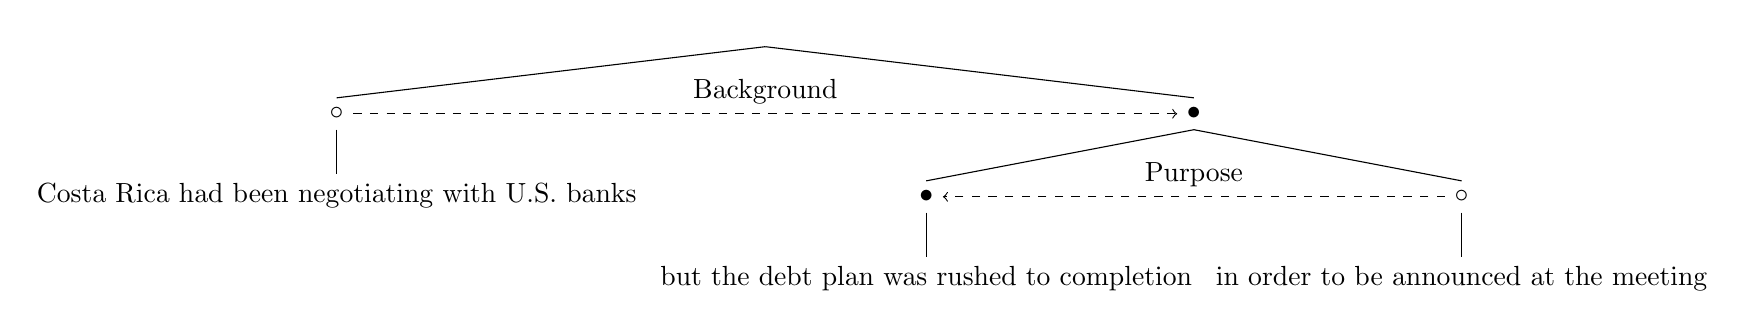
\begin{tikzpicture}
\Tree[.{} [.\node(a){$\circ$}; 
                               {Costa Rica had been negotiating with U.S. banks} ] 
          [.\node(b){$\bullet$}; [.\node(c){$\bullet$}; 
                                                        {but the debt plan was rushed to completion} ] 
                                 [.\node(d){$\circ$}; 
                                                      {in order to be announced at the meeting} ] ] ]
\draw[->, dashed] (a)-- node[above] {Background} ++(b);
\draw[->, dashed] (d)-- node[above] {Purpose} ++(c);
\end{tikzpicture}
}\\
(a) A discourse tree with 3 EDUs ($\bullet$: nucleas; $\circ$: satellite) in the RST treebank \cite{marcu2000theory}\\[0.2cm]
\resizebox{\textwidth}{!}{
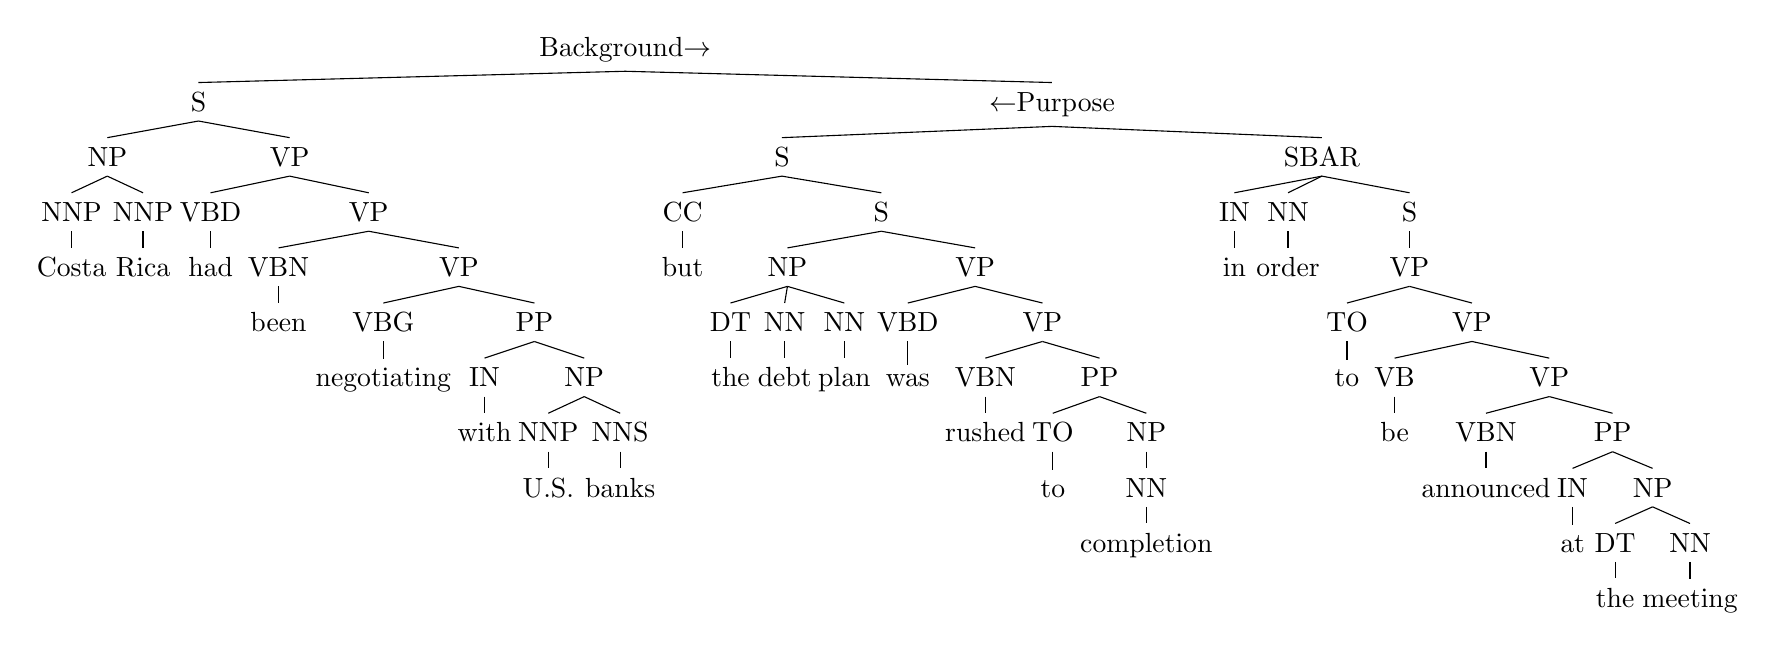
\begin{tikzpicture}
\tikzset{sibling distance=-0.15cm, level distance=.7cm}
\Tree[.{Background$\rightarrow$} [.S [.NP [.NNP Costa ] [.NNP Rica ] ]
                                     [.VP [.VBD had ]
                                          [.VP [.VBN been ] [.VP [.VBG negotiating ] 
                                                                 [.PP [.IN with ] 
                                                                      [.NP [.NNP U.S. ] [.NNS banks ] ] ]
                                                            ] ] ] ]
          [.{$\leftarrow$Purpose} [.S [.CC but ] 
                                      [.S [.NP [.DT the ] [.NN debt ] [.NN plan ]  ]
                                      [.VP [.VBD was ] 
                                           [.VP [.VBN rushed ] 
                                                [.PP [.TO to ] 
                                                     [.NP [.NN completion ]  ] ] ] ] ] ]
                                  [.SBAR [.IN in ] [.NN order ] 
                                                  [.S [.VP [.TO to ] 
                                                           [.VP [.VB be ] 
                                                                [.VP [.VBN announced ] 
                                                                     [.PP [.IN at ] 
                                                                          [.NP [.DT the ] [.NN meeting ]
                                                                          ] ] ] ] ] ] ] ] ]
\end{tikzpicture}
}\\[-0.3cm]
(b) The corresponding RST-PTB tree (our work)
\caption{Examples of the RST discourse treebank and our syntacto-discourse treebank (PTB-RST).\label{fig:rst-ptb}}
\end{figure*}
 
\begin{enumerate}
	\item We develop a combined representation of the constituency trees and discourse trees to facilitate 
	parsing at both levels without explicit conversion mechanism.
  Using this representation, we build and release a joint treebank based on the Penn
  Treebank \cite{marcus1993building} and RST Treebank \cite{marcu2000rhetorical,marcu2000theory}.
  (Section~\ref{sec:combined})
	\item We propose a novel joint parser that parses at both constituency and discourse levels.
	Our parser performs discourse parsing in an end-to-end manner, which greatly reduces
	the efforts required in preprocessing the text for segmentation and feature extraction,
	and, to our best knowledge, is the first end-to-end discourse parser in literature. (Section~\ref{sec:parsing})
	\item Following \newcite{cross2016incremental}, our incremental parser actually deos {\it not} require to design any explicit syntactic feature when predicting the output structure, thanks to the strong feature representing power of bi-directional LSTM.
	Besides this, our parser does not require binarization 
	of the discourse trees, which simplifies the parsing mechanism. (Section~\ref{sec:parsing})
	\item Empirical evaluations show that our end-to-end parser outperforms the traditional pipeline-based 
	discourse parsing algorithms. In ablation experiment, when the gold EDUs are provided, our parser is also competitive to other
	existing approaches with sophisticated features. (Section~\ref{sec:exps})
\end{enumerate}
 
\section{Combined Representation \& Treebank}\label{sec:combined}

We first briefly review the discourse trees in Rhetorical Structure Theory 
\cite{mann1988rhetorical},
and then discuss how to unify the discourse tree and constituency tree, 
which gives rise to our syntacto-discourse treebank PTB-RST.

\begin{figure*}[ht]
\centering
\resizebox{\textwidth}{!}{
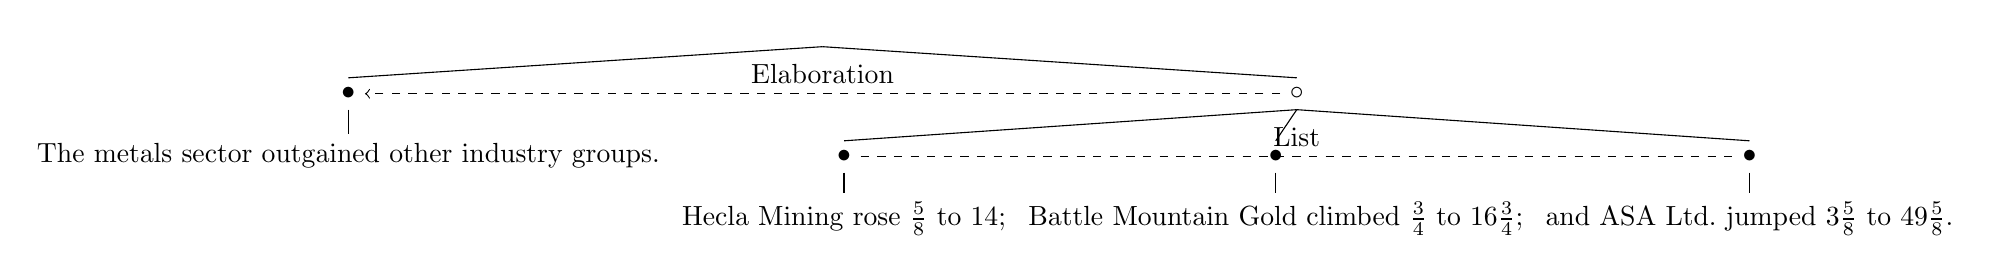
\begin{tikzpicture}
\tikzset{sibling distance=0.05cm, level distance=.8cm}
\Tree[.{} [.\node(a){$\bullet$}; 
                                 {The metals sector outgained other industry groups.} ] 
          [.\node(b){$\circ$}; [.\node(c){$\bullet$}; 
                                                      {Hecla Mining rose $\frac{5}{8}$ to 14;} ] 
                               [.\node(d){$\bullet$}; 
                                                      {Battle Mountain Gold climbed $\frac{3}{4}$ to 16$\frac{3}{4}$;} ] 
                               [.\node(e){$\bullet$}; 
                                                      {and ASA Ltd.~jumped 3$\frac{5}{8}$ to 49$\frac{5}{8}$.} ] 
          ] 
     ]
\draw[->, dashed] (b)-- node[above] {Elaboration} ++(a);
\draw[-, dashed] (c)-- node[above] {List} ++(e);



\end{tikzpicture}
}\\[0.1cm]

\resizebox{\textwidth}{!}{
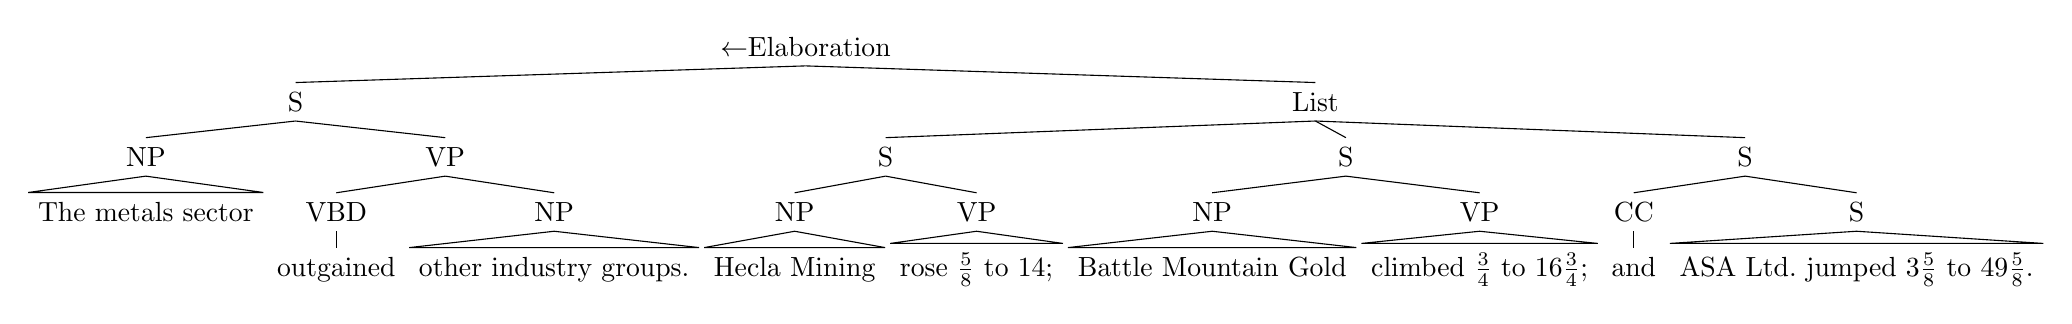
\begin{tikzpicture}
\tikzset{sibling distance=0.05cm, level distance=.7cm}
\Tree [.{$\leftarrow$Elaboration} 
        [.S 
          [.NP \edge[roof]; {The metals sector} ]
          [.VP 
            [.VBD outgained ]
            [.NP \edge[roof]; {other industry groups.} ]
          ]
        ]
        [.{List}
          [.S 
            [.NP \edge[roof]; {Hecla Mining} ]
            [.VP \edge[roof]; {rose $\frac{5}{8}$ to 14;} ]
          ]
          [.S 
            [.NP \edge[roof]; {Battle Mountain Gold} ]
            [.VP \edge[roof]; {climbed $\frac{3}{4}$ to 16$\frac{3}{4}$;} ]
          ]
          [.S 
            [.CC and ]
            [.S \edge[roof]; {ASA Ltd.~jumped 3$\frac{5}{8}$ to 49$\frac{5}{8}$.} ]
          ]
        ]
      ]
\end{tikzpicture}
}\\[-0.3cm] 
\caption{
Another example of RST vs.~PTB-RST, demonstrating
a discourse tree over two sentences and a non-binary relation (List).
The lower levels of the PTB-RST tree are collapsed due to space contraints.
\label{fig:secondexample}}
\vspace{-0.7cm}
\end{figure*}

 


\subsection{Review: RST Discourse Tree}

In RST, 
structure, i.e., the discourse tree.
There are two types of branchings in a discourse tree. 
Most of the internal discourse tree
nodes are binary branching, with one {\it nucleus} child 
containing the core semantic meaning of the current node, 
and one {\it satellite} child semantically decorating 
the nucleus. Like dependency labels,
there is a {\em relation} annotated 
between each satellite-nucleus pair, 
such as ``Background'' or ``Purpose''.
Figure~\ref{fig:rst-ptb}(a) shows an example RST tree.
There are also non-binary-branching internal nodes whose children are conjunctions, e.g., a ``List'' of semantically similar
EDUs (which are all nucleus nodes); see Figure~\ref{fig:secondexample}(a) for an example.

\subsection{Syntacto-Discourse Representation}

It is widely recognized that lower-level lexical and syntactic information can greatly help 
determining both the boundaries of the EDUs 
(i.e., discourse segmentation) \cite{bach2012reranking} 
as well as the semantic relations between EDUs 
\cite{soricut2003sentence,hernault2010hilda,joty2014discriminative,feng2014linear,ji2014representation,li2014recursive,heilman2015fast}.
While these previous approaches 
rely
on pre-trained tools to provide 
both EDU segmentations and
intra-EDU syntactic parse trees,
we instead propose to directly determine 
the low-level segmentations,
the syntactic parses,
and the high-level discourse parses
using a single joint parser.
This parser is trained on the combined trees of constituency 
and discourse structures.


We first convert the RST trees to the constituency tree structures as defined in the Penn Treebank \cite{marcus1993building}.
For each binary branching node with a nucleus child and a satellite child, we use the relation as the label of the converted
parent node. The nucleus/satellite relation 
(either $\leftarrow$ or $\rightarrow$, pointing from satellite to nucleus) 
is then attached to the label as a suffix.
For example, the top level relation in Figure~\ref{fig:secondexample},
\begin{center}
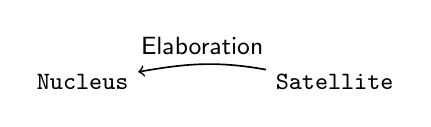
\begin{tikzpicture}[font=\small,scale=0.8]
\node (a) at (0, 0) {\tt Nucleus};
\node (b) at (4, 0) {\tt Satellite};
\draw[->, semithick] (b) to [out=170, in=10] node[above]{\sf Elaboration} (a);
\end{tikzpicture}
\end{center}
is converted into
\begin{center}
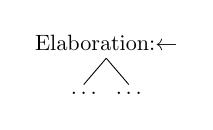
\begin{tikzpicture}[level distance=20,scale=0.8]
\Tree [.{Elaboration:$\leftarrow$} {$\ldots$} {$\ldots$} ]
\end{tikzpicture}
\end{center}
For each conjunctive branch, we simply use the relation as the label of the converted parent node. 

After converting the RST trees into constituency tree format, we then align the constituency trees for each EDU span to the converted 
discourse tree leaves. Given that the RST Treebank \cite{marcu2000theory} is a subset of the Penn Treebank,
we can always find the corresponding constituency subtrees for each EDU leaf node.
For the most cases, each EDU corresponds to one single (sub)tree in the Penn Treebank, since the semantic units 
highly correlate with the syntactic units. 
In some other cases, one EDU leaf node may correspond to multiple subtrees in the Penn Treebank,
and for these EDUs we simply treat them as multiple-branching nodes in the converted trees.

Figure~\ref{fig:secondexample} shows an example of a discourse tree and its combined tree.


\begin{figure}
\centering
\includegraphics[width=0.33\textwidth,height=2.6cm]{lendistr.pdf}\\[-0.3cm]
\caption{PTB-RST: length distribution (\# tokens).\label{fig:treelen}}
\end{figure}


\subsection{Joint Treebank}

Using the conversion strategy described in the previous subsection, we build the first joint
syntactic and discourse
treebank based on Penn Treebank \cite{marcus1993building} and RST Treebank \cite{marcu2000rhetorical,marcu2000theory}.
This treebank is released as a set of tools to generate the joint trees 
given Penn Treebank and RST Treebank data.
During the alignment between the RST trees and the constituent trees,
we only keep the common parts of the two trees.

We follow the training/testing splitting strategy of RST Treebank.
In the training set, there are 347 joint trees with 
17,837 tokens in total,
in which the lengths of the discourses
vary from 30 to 2,199.
In the testing set, there are 38 joint trees
with 4,819 tokens in total,
in which the lengths of the discourses
vary from 45 to 2,607.
Figure~\ref{fig:treelen} shows the distribution of the discourse lengths
over the whole dataset.

 
\section{Joint Syntacto-Discourse Parsing}\label{sec:parsing}


Given the combined syntactic and discourse treebank, we now propose a joint parser
that can perform end-to-end discourse parsing. 
Later in this section we will briefly discuss the underlying recurrent neural models
and the training of the parser.

\subsection{Extending Span-based Parsing}

\begin{figure}
\hspace{-0.4cm}
\resizebox{0.53\textwidth}{!}{
  \begin{tabular}{cl}
   input      & $w_0 \ldots w_{n-1}$ \\[0.1in]
    axiom    & \tuple{\ _{-1} \trivialtrapezoid _0}: $(0, \emptyset)$ \quad    goal  \quad \tuple{\ _{-1} \trivialtrapezoid _0 \trapezoid _n}: $(\_, t)$ \\[0.1in]
    \shift   & $\inferrule{\tuple{ ...\ _i \trapezoid _j}: (c, t)}
                          {\tuple{... \ _i \trapezoid _j \shorttrapezoid{j} _{j+1}}: (c+\scoreshift{i, j}, t)}$ $j<n$ \\[0.25in]
    \comb    & $\inferrule{\tuple{ ... \ _i \trapezoid _k \trapezoid _j}: (c, t) }
                          {\tuple{... \ _i \longtrapezoid{k} _j}: (c + \scorecomb{i, k, j}, t)}$ \\[0.25in]
    \labelx  & $\inferrule{\tuple{... \ _i \longtrapezoid{k} _j}: (c, t)}
                          {\tuple{ ... \ _i \trapezoid _j}: (c+\scorelabelx{i, k, j}, t\cup\{_i X_j\})} $ \\[0.25in]
    \nolabel & $\inferrule{\tuple{... \ _i \longtrapezoid{k} _j}: (c, t)}
                          {\tuple{ ... \ _i \trapezoid _j}: (c +\scorenolabel{i,k,j}, t)}$ 
  \end{tabular}
  }
\caption{Deductive system for joint syntactic and discourse parsing. 
$\scoreshift{\cdot, \cdot}$, $\scorecomb{\cdot, \cdot, \cdot}$, 
$\scorelabelx{\cdot, \cdot, \cdot}$, and $\scorenolabel{\cdot, \cdot, \cdot}$ are 
scoring functions evaluated in the neural network.}
\label{fig:sr}
\end{figure}




Due to efficiency considerations for a long sequence of words in a document, 
we resort to incremental parsing.
The deductive system for our joint parsing algorithm (Figure~\ref{fig:sr}) is inspired by 
the span-based constituency parser of \newcite{cross2016incremental}.

At each parsing step, we maintain a configuration that is a triple $\tuple{z, \sigma, k}$, 
where $z$ is the number of parsing actions performed, 
$\sigma$ is a stack, and $k$ is the previous branching position.
In traditional incremental parsing, the stack $\sigma$ stores the subtrees that have been constructed
during the parsing. However, in the span-based constituency parsing, the stack $\sigma$ only needs
to store the boundaries of the subtrees, which are actually a list of indexes representing the spans of the subtrees.
Please refer \newcite{cross2016incremental} for details of the span-based constituency parsing.

The actions we can perform at each step is conditioned on whether the current step is even or odd.
For even steps, we perform structural actions, i.e., either shift (\shift) or combine (\comb);
and for odd steps, we perform label actions, i.e., either mark the top span with a label, or 
mark a \nolabel for multiple branching nodes.

Different from \newcite{cross2016incremental}, in the combine action, we choose to keep the last 
branching point $k$. This is because in our parsing mechanism,
the discourse relation between two EDUs is actually determined after the previous combine action.
We need to keep the splitting point to clearly find the spans of the two EDUs to determine their relations.

The \nolabel action makes the binarization of the discourse/constituency tree unnecessary,
because \nolabel actually combines the top two spans on the stack $\sigma$ into one span,
but without annotating the new span a label.
This greatly simplifies the pre-processing and post-processing efforts needed.


\begin{table}
  \begin{center}
  \resizebox{0.35\textwidth}{!}{
  \begin{tabular}{c|c|c|c}
    & Prec. & Recall & F1 \\
    \hline
    \hline
    Constituency & 87.6 & 86.9 & 87.2 \\
    Discourse & 46.5 & 40.2 & 43.0 \\
    \hline
    Overall & 83.5 & 81.6 & 82.5
  \end{tabular}
  }
  \end{center}
  \caption{Accuracies on PTB-RST at constituency and discourse levels. 
    \label{tab:internal-acc}
  }
  \vspace{-0.4cm}
\end{table}

Note that our parser actually does not rely on any explicit syntactic features when predicting
the discourse-level structures and labels. It predicts sololy based
on the span feature representations from underlying bi-directional LSTM.

\begin{table*}
\begin{center}
\resizebox{0.9\textwidth}{!}{
\begin{tabular}{c|c|c|c|ccc}
& description & syntactic feats. & segmentation & structure & +nuclearity & +relation \\
\hline\hline
\newcite{bach2012reranking} &segmentation only & Stanford & 95.1 & - & - & -\\
\hline
\newcite{hernault2010hilda} & end-to-end pipeline & Penn Treebank & 94.0 & 72.3 & 59.1 & 47.3 \\
\hline
\multicolumn{2}{c|}{joint syntactic \& discourse parsing } & - & {\bf 95.4} & {\bf 78.8} & {\bf 65.0} & {\bf 52.2}\\
\end{tabular}
}
\end{center}
\caption{F1 scores of end-to-end systems. ``+nuclearity'' 
indicates scoring of tree structures with nuclearity included. 
``+relation'' has both nuclearity and relation included (e.g., $\leftarrow$Elaboration).
\label{tab:results} }
\vspace{-0.4cm}
\end{table*}

 \begin{table*}
\begin{center}
\resizebox{0.9\textwidth}{!}{
\begin{tabular}{c|c|c|ccc}
& & syntactic feats &  structure & +nuclearity & +relation \\
\hline
\multicolumn{2}{c|}{human annotation \cite{ji2014representation}} & - & 88.7 & 77.7 & 65.8\\
\hline\hline
\multirow{5}{*}{sparse} &\newcite{hernault2010hilda} & Penn Treebank&  83.0 & 68.4 & 54.8\\
&\newcite{joty2013combining} & Charniak (retrained) &82.7 & 68.4 & 55.7\\
&\newcite{joty2014discriminative} &  Charniak (retrained) & - & - & 57.3\\
&\newcite{feng2014linear} &  Stanford &85.7 & 71.0 & 58.2\\
&\newcite{heilman2015fast} &  ZPar (retraied)&83.5 & 68.1 & 55.1\\
&\newcite{wang2017two} & Stanford & {\bf 86.0} & {\bf 72.4} & 59.7 \\
\hline
\multirow{4}{*}{neural} &\newcite{li2014recursive} & \multirow{2}{*}{Stanford} &82.4 & 69.2 & 56.8 \\
&+ sparse features &  &84.0 & 70.8 & 58.6 \\
&\newcite{ji2014representation} & \multirow{2}{*}{MALT} & 80.5 & 68.6 & 58.3\\
&+ sparse features &  &81.6 & 71.1 & {\bf 61.8}\\
\hline\hline
 &span-based discourse parsing & - & 84.2 & 67.7 & 56.0
\end{tabular}
}
\end{center}
\caption{Experiments using gold segmentations.
The column of ``syntactic feats'' shows how the syntactic features
are calculated in the corresponding systems. Note that our parser
predicts solely based on the span features from bi-directionaly LSTM,
instead of any explicitly designed syntactic features.
\label{tab:results-gold} }
\end{table*}
 
\subsection{Recurrent Neural Models and Training}

The scoring functions in the deductive system (Figure~\ref{fig:sr})
are calculated by an underlying neural model,
which is similar to the bi-directional LSTM model
in \newcite{cross2016incremental} that evaluates based on span boundary features.

During the decoding time, 
a document is firstly passed into a two-layer bi-directional LSTM
model, then the outputs at each text position of the two layers of the bi-directional
LSTMs are concatenated as the positional features.
The spans at each parsing step can be represented as the feature vectors at the boundaries.
The span features are then passed into fully connected networks with softmax to calculate the 
likelihood of performing the corresponding action or marking the corresponding label.

We use the ``training with exploration'' strategy \cite{goldberg2013training}
and the dynamic oracle mechanism described in \newcite{cross2016incremental}
to make sure the model can handle unseen parsing configurations properly.


 
\section{Empirical Evaluations}\label{sec:exps}


We use the treebank described in Section~\ref{sec:combined}
for empirical evaluation.
We randomly choose 30 documents from the training set as the development set.


We tune the hyperparameters of the neural model on the development set.
For most of the hyperparameters we settle with the same values
suggested by \newcite{cross2016incremental}.
To alleviate the overfitting problem for training on the relative small
RST Treebank, we use a dropout of 0.5.

One particular hyperparameter is that we use a value $\beta$ to
balance the chances between training following the exploration (i.e., the best action
chosen by the neural model)
and following the correct path provided by the dynamic oracle.
We find that $\beta=0.8$, i.e., following the dynamic oracle
with a probability of 0.8, achieves the best performance.
One explanation for this high chance to follow the oracle is that, since our combined trees are significantly larger 
than the constituency trees in Penn Treebank,
lower $\beta$ makes the parsing easily divert into wrong trails that are difficult to learn from.

Since our parser essentially performs both constituency parsing task and discourse parsing task.
We also evaluate the performances on sentence constituency level and
discourse level separately. The result is shown in Table~\ref{tab:internal-acc}.
Note that in constituency level, the accuracy is not directly comparable with the accuracy
reported in \newcite{cross2016incremental}, since:
a) our parser is trained on a much smaller dataset (RST Treebank
is about 1/6 of Penn Treebank); b) the parser is trained to optimize
the discourse-level accuracy.

Table~\ref{tab:results} shows that, 
in the perspective of end-to-end discourse parsing,
our parser first outperforms the state-of-the-art segmentator
of \newcite{bach2012reranking},
and furthermore, in end-to-end parsing, the superiority
of our parser is more pronounced comparing to
the previously best parser of \newcite{hernault2010hilda}.

On the other hand, the majority of the conventional discourse parsers are not end-to-end:
they rely on gold EDU segmentations and pre-trained tools like Stanford parsers to generate features.
We perform an experiment to compare the performance of our parser
with them given the gold EDU segments (Table~\ref{tab:results-gold}).
Note that most of these parsers do not handle multi-branching discourse nodes and are trained and evaluated
on binarized discourse trees \cite{feng2014linear,li2014recursive,li2014text,ji2014representation,heilman2015fast}, so their performances are actually not directly comparable to
the results we reported.


\iffalse
We also noticed that for neural models, some sparse features,
like lengths of EDUs, distances between EDUs, and whether two EDUs are in the same sentence,
can significantly improve the parsing performance in nuclearity and relation,
and they are difficult for the neural models to extract \cite{li2014recursive,ji2014representation}.
\fi
 
\section{Conclusion}
We have presented a neural-based incremental parser that can jointly parse
at both constituency and discourse levels.
To our best knowledge, this is the first end-to-end parser for discourse parsing task.
Our parser achieves the state-of-the-art performance in end-to-end parsing,
and unlike previous approaches, needs little pre-processing effort.

\section*{Acknowledgments}
{\small
We thank the anonymous reviewers for helpful comments.
We are also grateful to Mingbo Ma, James Cross, and Dezhong Deng for suggestions.
This work is supported in part by
NSF IIS-1656051,
DARPA N66001-17-2-4030 (XAI),
a Google Faculty Research Award,
and an HP Gift.
}
\bibliography{emnlp2017}
\bibliographystyle{emnlp_natbib}

\end{document}
